\documentclass[11pt]{article}

% ---------------------------------------------------------------------------
% QAPINN-BQP  --  Extended Technical Report (working / planning version)
% = the submission report PLUS future work, roadmap, and scope boundaries.
% WISER Global Quantum+AI Program 2026  --  BQP Challenge
% Compile: pdflatex qapinn_report_extended.tex  (twice)
% ---------------------------------------------------------------------------

\usepackage[margin=1in]{geometry}
\usepackage{graphicx}
\usepackage{amsmath,amssymb}
\usepackage{booktabs}
\usepackage{multirow}
\usepackage{xcolor}
\usepackage[hidelinks]{hyperref}
\usepackage{caption}
\usepackage{subcaption}
\usepackage{enumitem}

\graphicspath{{../results/}{../results/ablation_summary/}{../results/_montage/}{../results/reference/}}

\newcommand{\todo}[1]{\textcolor{blue}{\textbf{[TODO: #1]}}}

\title{\textbf{Explaining the Quantum Layer in Physics-Informed Neural Networks:\\
A Spectral and Mechanistic Study \\[2pt] \large (Extended / Working Report with Roadmap)}}
\author{WISER Global Quantum+AI Program 2026 --- BQP Challenge\\
\emph{Quantum-Assisted Physics-Informed Neural Networks for CFD}}
\date{Draft --- July 2026}

\begin{document}
\maketitle

\begin{abstract}
This is the extended working version of the QAPINN-BQP report. It contains the
full technical content of the submission draft --- a verified parameter-matched
test bench, a five-dimension explainability suite, and a Tier-1 ablation on
Burgers --- and additionally documents the \emph{complete experimental roadmap},
the statistical work required to promote our current single-seed hypotheses to
claims, and an explicit account of everything currently \emph{left out} of scope.
Headline hypotheses (single seed, one undertrained PDE): a QAPINN's advantage
tracks the frequency-setting knobs (depth, qubits, encoding scale), not
\emph{entanglement} at fixed band; and against a structurally-identical
classical-front-end control the advantage is \emph{bandwidth-gated} while the
apparent classical-side effects (neuron diversity, gradient amplification) do
\emph{not} survive --- what remains is a bandwidth-gated advantage and a
barren-plateau signature in qubit count. The pipeline is independently verified
(8/8 checks); the conclusions are
not yet, and the path to establishing them is the subject of Sections
\ref{sec:roadmap}--\ref{sec:leftout}.
\end{abstract}

\tableofcontents
\newpage

% ===========================================================================
\section{Introduction}
Physics-Informed Neural Networks (PINNs)~\cite{raissi} make the differential
equation the loss. A Quantum-Assisted PINN (QAPINN)~\cite{qapinn} replaces the
first hidden layer with a variational quantum circuit (VQC), and is reported to cut
trainable parameters at maintained accuracy. The BQP challenge asks us to
\emph{explain} the learning dynamics --- when, why, and how the quantum layer
changes learning --- and to derive a problem-specific circuit-design methodology.

We adopt the dominant theoretical lens for VQCs (a data-encoding circuit is a
truncated Fourier series~\cite{schuld}) and test whether it suffices to explain a
QAPINN's behaviour, and how the quantum layer changes the classical network it is
attached to. Contributions and results mirror the submission report; the extended
value here is the roadmap (Sec.~\ref{sec:roadmap}) and scope boundaries
(Sec.~\ref{sec:leftout}).

% ===========================================================================
\section{Background and Related Work}
A VQC with data-encoding gates is a partial Fourier series
$f(x)=\sum_{\omega\in\Omega}c_\omega e^{i\omega x}$: the frequency set $\Omega$ is
fixed by the encoding (with $L$ re-uploads, $\Omega=\{-L,\dots,L\}$), the
coefficients $c_\omega$ by the trainable gates~\cite{schuld}. Mhiri
et al.~\cite{mhiri} show the coefficients are additionally constrained and can
vanish with qubit count --- frequencies are necessary but not sufficient.
Differentiable quantum circuits solve DEs with analytic
derivatives~\cite{dqc}; hybrid QAPINN/QCPINN designs~\cite{qapinn,qcpinn} report
PDE-dependent parameter reduction (quantum sometimes \emph{loses}, e.g.\ cavity
flow); a ``black-hole'' collapse to the trivial solution is a distinct trainability
pathology~\cite{maxwell}. No validated mechanism explains \emph{when/why} the
quantum layer helps --- the gap targeted here.

% ===========================================================================
\section{Methodology}
\subsection{Test problems}
Same domain, IC $u(x,0)=-\sin(\pi x)$, and BCs for both PDEs, so only the operator
differs: Burgers $u_t+u u_x=\nu u_{xx}$ ($\nu=0.01/\pi$, shock $\to$ broadband)
with an exact Cole--Hopf reference (Fig.~\ref{fig:reference}); heat $u_t=\alpha
u_{xx}$ ($\alpha=1/\pi^2$, single mode $u=-\sin(\pi x)e^{-t}$).

\begin{figure}[t]
  \centering
  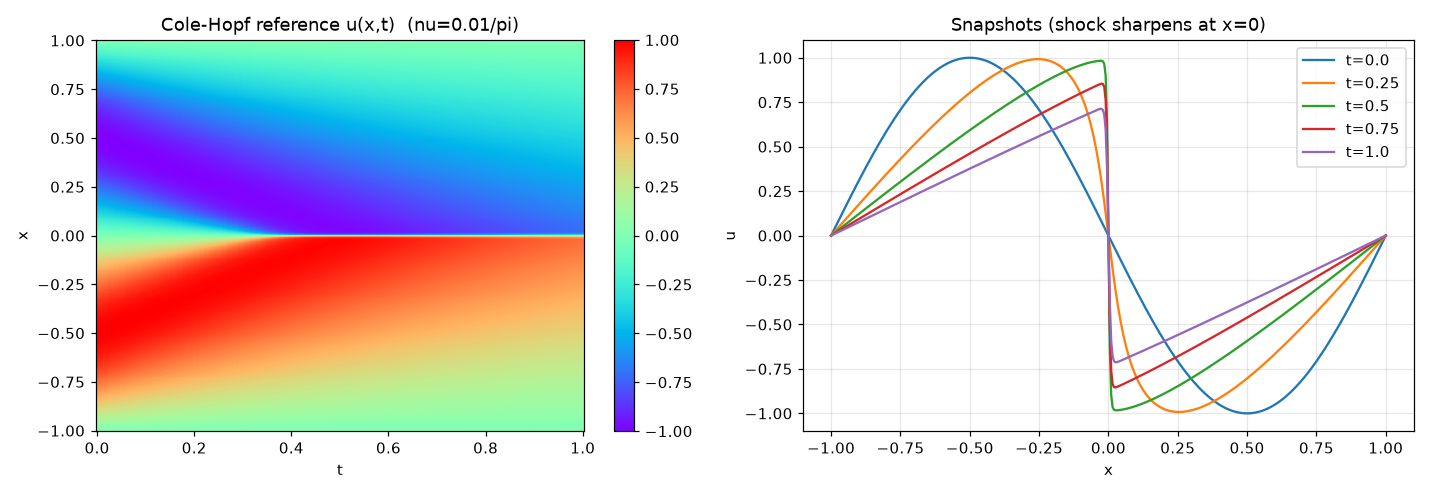
\includegraphics[width=0.9\textwidth]{burgers_reference.png}
  \caption{Exact Cole--Hopf Burgers reference: field (left) and snapshots (right),
  showing the shock at $x=0$.}
  \label{fig:reference}
\end{figure}

\subsection{Models and XAI suite}
Classical PINN ($\tanh$ MLP) vs QAPINN (fixed coord-map $\to$ VQC $\to$ classical
post-net), compared at matched parameters. Baseline VQC: 4 qubits, depth 3, $RY$
re-uploading, linear CNOT chain, $\langle Z_i\rangle$ measurement, post-net $[16]$
(121 params, 24 quantum). Five XAI dimensions (spectral/F-principle; neurons;
VQC internals incl.\ entanglement entropy; loss landscape; generalisation) plus
training-time spectrum and per-layer/per-qubit gradient-variance probes.

\subsection{Verification}
All eight independent correctness checks pass (Table~\ref{tab:verify}); notably,
the VQC is confirmed to be a truncated Fourier series with maximum frequency equal
to the re-upload depth.

\begin{table}[t]
  \centering \small
  \begin{tabular}{lll}
    \toprule
    Check & Method & Result \\ \midrule
    Burgers residual & vs analytic & $1.2\times10^{-7}$ \\
    Heat residual & exact $\to$ residual & $6.0\times10^{-8}$ \\
    Autograd $u_x$ & vs finite diff & match \\
    VQC = Fourier, max freq $=$ depth & $L{=}2\!\to\!2,\ L{=}4\!\to\!4$ & pass \\
    relative-$L_2$ & exact $\to 0$ & $4.0\times10^{-8}$ \\
    Matched params & all configs & 121 \\
    Reproducibility & same seed & bit-exact \\ \bottomrule
  \end{tabular}
  \caption{Correctness audit (8/8).}
  \label{tab:verify}
\end{table}

% ===========================================================================
\section{Experiments and Results}
\subsection{Baseline and spectra}
At 121 matched params (Adam, 2000 iters, seed 0): heat solved by both (classical
$8.3\!\times\!10^{-3}$, QAPINN $5.9\!\times\!10^{-3}$); Burgers undertrained
(classical $0.433$, QAPINN $0.472$). Spectra (Fig.~\ref{fig:spectrum}): heat is a
single $k{=}1$ mode; Burgers is broadband and both models undershoot the high
harmonics (depth-3 VQC capped near $k\!\approx\!3$).

\begin{figure}[t]
  \centering
  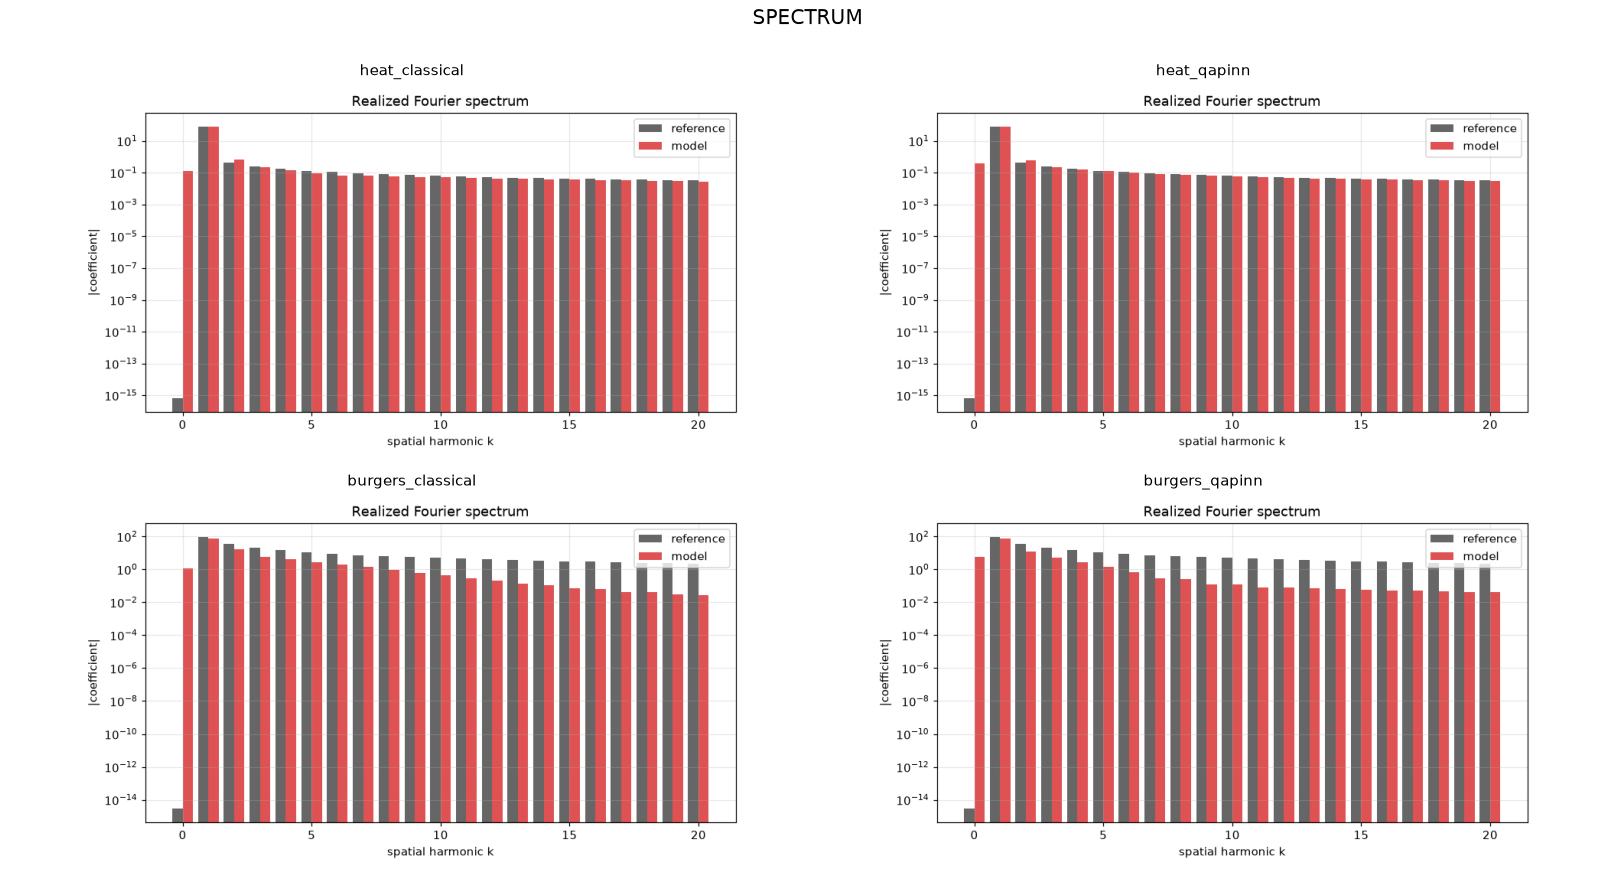
\includegraphics[width=\textwidth]{spectrum.png}
  \caption{Realised spectra (grey reference, red model). Burgers (bottom): both
  models undershoot the high-frequency shock tail.}
  \label{fig:spectrum}
\end{figure}

\subsection{Tier-1 ablation}
\textbf{Depth $=$ bandwidth} (Fig.~\ref{fig:depth}): QAPINN accuracy improves
monotonically ($0.57\!\to\!0.42$), matched classical stays flat; realised max
harmonic grows with depth; QAPINN overtakes classical at depth $\geq3$.
\textbf{Entanglement at fixed band} (Fig.~\ref{fig:ent}): accuracy barely moves
($0.456$--$0.488$), \emph{more} entanglement slightly \emph{worse}, none is best
--- contradicting entanglement-driven expressibility. \textbf{Post-net width}: the
VQC needs a readout but beats matched classical for any post-net $\geq[8]$.

\begin{figure}[t]
  \centering
  \begin{subfigure}{0.49\textwidth}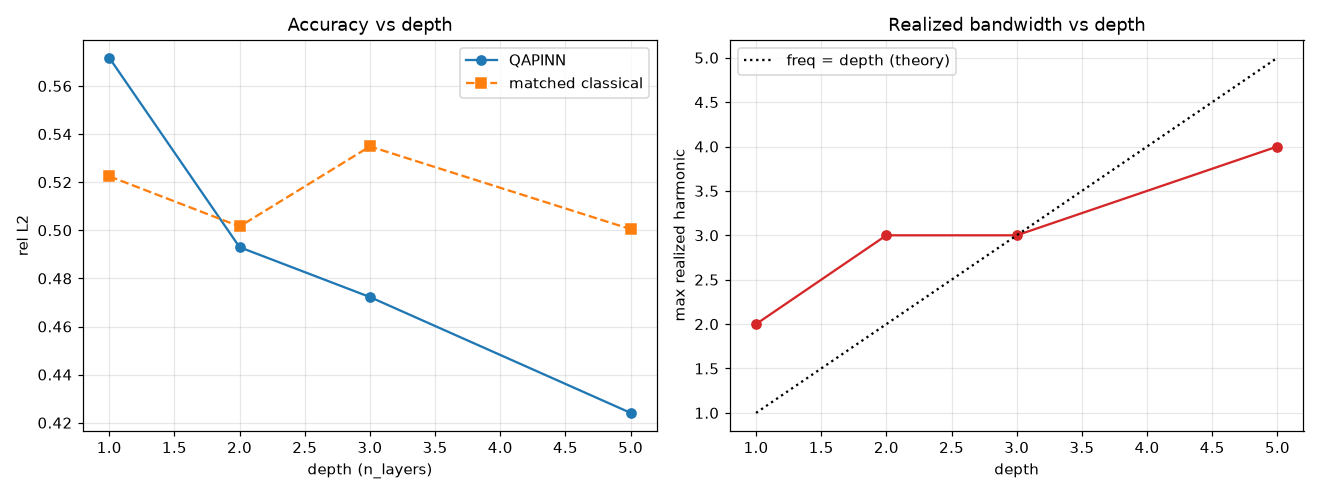
\includegraphics[width=\textwidth]{depth_sweep.png}\caption{Depth.}\label{fig:depth}\end{subfigure}\hfill
  \begin{subfigure}{0.49\textwidth}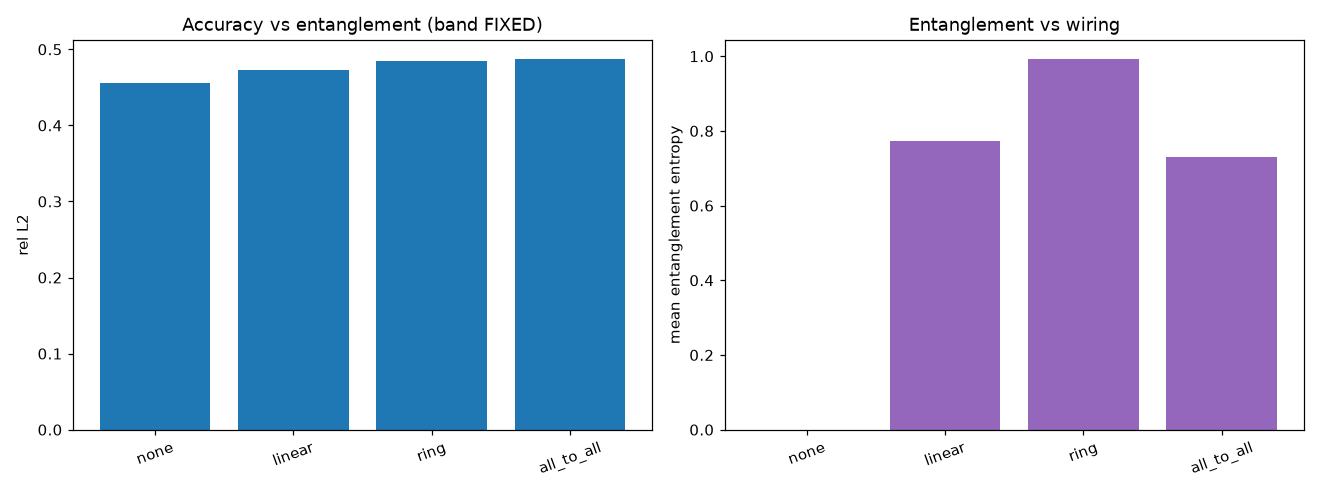
\includegraphics[width=\textwidth]{entanglement_sweep.png}\caption{Entanglement (band fixed).}\label{fig:ent}\end{subfigure}
  \caption{Tier-1 ablations on Burgers.}
\end{figure}

\begin{table}[t]
  \centering \small
  \begin{tabular}{llccc}
    \toprule
    Sweep & Config & Params & QAPINN rel-$L_2$ & matched classical rel-$L_2$ \\
    \midrule
    \multirow{4}{*}{Depth}
      & $L=1$ & 105 & 0.572 & 0.522 \\
      & $L=2$ & 113 & 0.493 & 0.502 \\
      & $L=3$ (baseline) & 121 & 0.472 & 0.535 \\
      & $L=5$ & 137 & \textbf{0.424} & 0.500 \\
    \midrule
    \multirow{4}{*}{\shortstack[l]{Entanglement\\(band fixed)}}
      & none & 121 & \textbf{0.456} & 0.535 \\
      & linear & 121 & 0.472 & 0.535 \\
      & ring & 121 & 0.485 & 0.535 \\
      & all-to-all & 121 & 0.488 & 0.535 \\
    \midrule
    \multirow{4}{*}{Post-net}
      & $[\,]$ (linear) & 29 & 0.544 & 0.533 \\
      & $[8]$ & 73 & 0.478 & 0.533 \\
      & $[16]$ (baseline) & 121 & 0.472 & 0.535 \\
      & $[32]$ & 217 & \textbf{0.466} & 0.505 \\
    \bottomrule
  \end{tabular}
  \caption{Complete Tier-1 ablation results (single seed, Burgers, 2000 Adam
  iters). QAPINN improves with depth and post-net width and overtakes the matched
  classical control; at fixed band, entanglement does not help (\emph{none} best).}
  \label{tab:ablation}
\end{table}

\begin{figure}[t]
  \centering 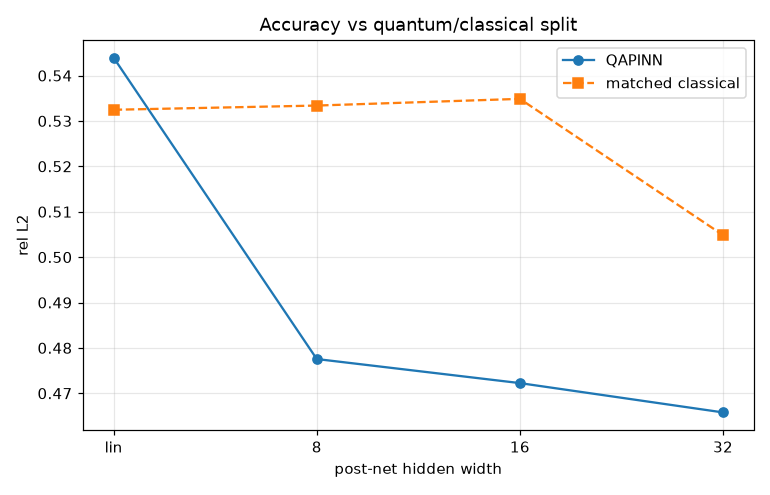
\includegraphics[width=0.55\textwidth]{post_sweep.png}
  \caption{Post-net width sweep: QAPINN vs matched classical. The VQC needs a small
  readout but beats matched classical for any post-net $\geq[8]$.}
  \label{fig:post}
\end{figure}

\begin{figure}[t]
  \centering 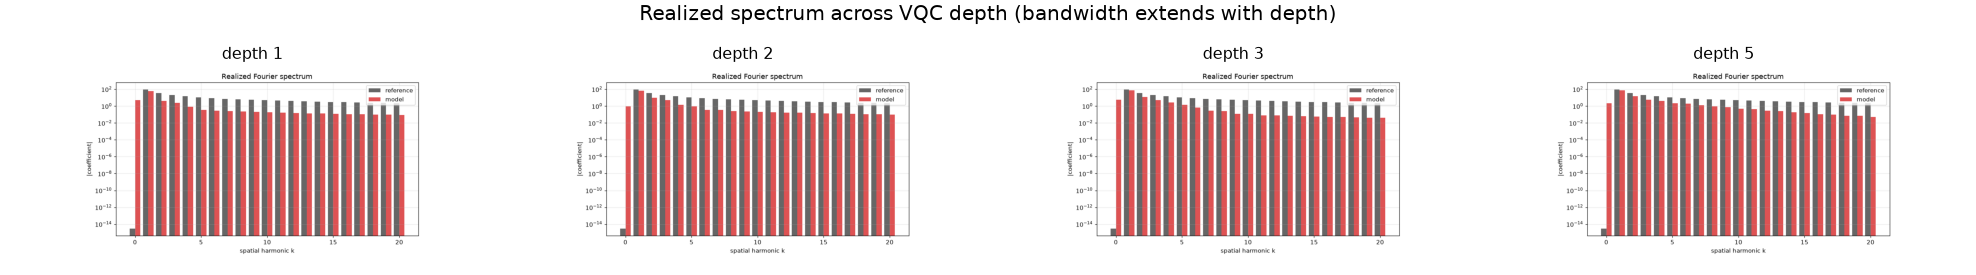
\includegraphics[width=\textwidth]{depth_spectra.png}
  \caption{Realised spectrum (grey reference, red model) across VQC depth --- the
  model captures more of the high-frequency shock tail as depth grows.}
  \label{fig:depthspec}
\end{figure}

\begin{figure}[t]
  \centering 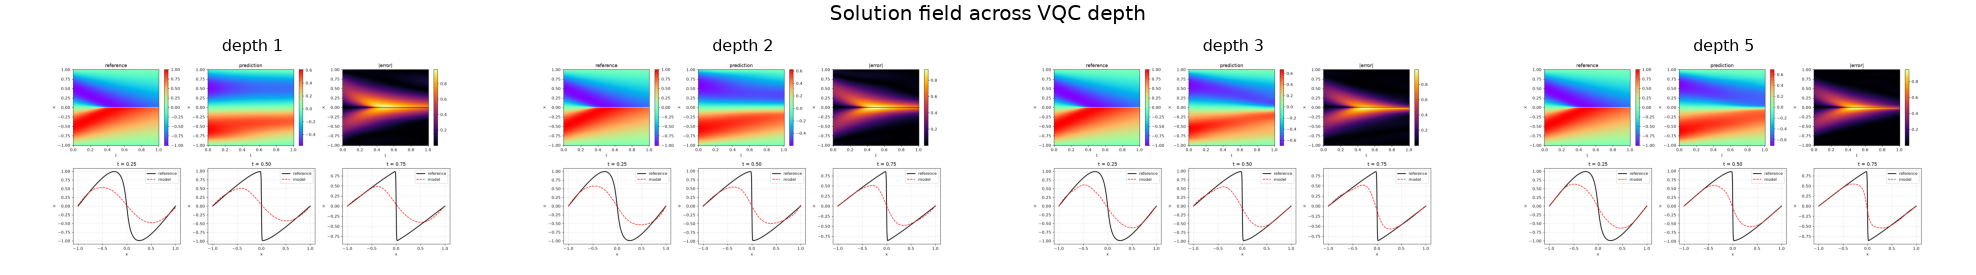
\includegraphics[width=\textwidth]{depth_solutions.png}
  \caption{QAPINN solution field across VQC depth.}
  \label{fig:depthsol}
\end{figure}

\begin{figure}[t]
  \centering 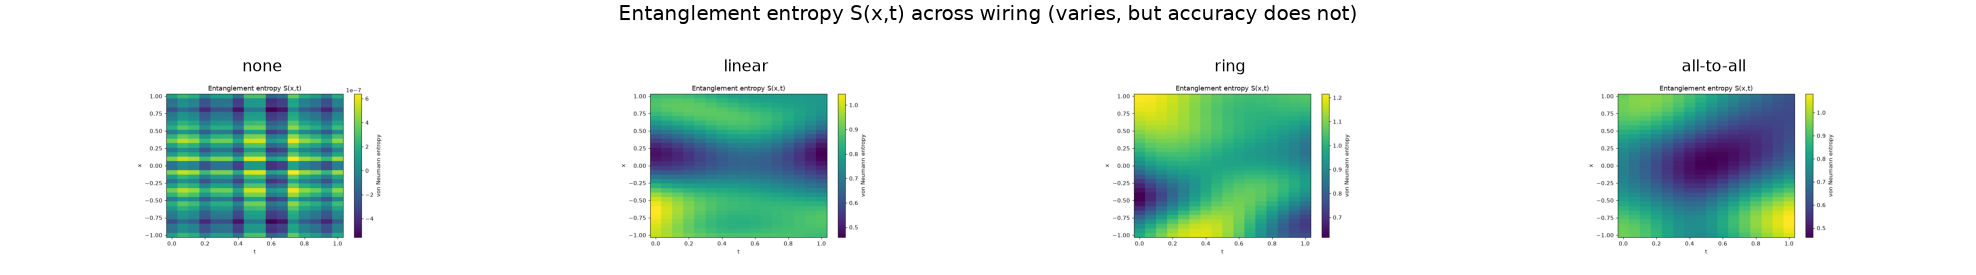
\includegraphics[width=\textwidth]{ent_entropy_fields.png}
  \caption{Entanglement entropy $S(x,t)$ across entangling patterns: entropy varies
  strongly while accuracy does not (Table~\ref{tab:ablation}).}
  \label{fig:entfields}
\end{figure}

\subsection{Tier-3 ablation: qubits, measurement, encoding scale}
The remaining knobs (Table~\ref{tab:tier3}, Fig.~\ref{fig:tier3}) reinforce the
picture. \textbf{Qubits} behave like depth: accuracy improves monotonically
($0.501\!\to\!0.443$), QAPINN overtakes matched classical at $\geq4$ qubits.
\textbf{Measurement:} single $\langle Z_0\rangle$ bottlenecks ($0.591$); multi $=$
$ZZ$ ($0.472$) --- readout width matters, correlator type does not.
\textbf{Encoding scale:} optimum near $1.0$, catastrophic collapse to the trivial
solution at $2\pi$ --- the black-hole pathology as an ablation.

\begin{table}[t]
  \centering \small
  \begin{tabular}{llccc}
    \toprule
    Sweep & Config & Params & QAPINN rel-$L_2$ & matched cls.\ rel-$L_2$ \\ \midrule
    \multirow{4}{*}{Qubits}
      & 3 & 99 & 0.501 & 0.470 \\
      & 4 (base) & 121 & 0.472 & 0.535 \\
      & 5 & 143 & 0.468 & 0.541 \\
      & 6 & 165 & \textbf{0.443} & 0.465 \\ \midrule
    \multirow{3}{*}{Measure}
      & single & 73 & 0.591 & 0.533 \\
      & multi (base) & 121 & 0.472 & 0.535 \\
      & $ZZ$ & 169 & 0.472 & 0.515 \\ \midrule
    \multirow{4}{*}{input\_scale}
      & 0.5 & 121 & 0.513 & 0.535 \\
      & 1.0 (base) & 121 & \textbf{0.472} & 0.535 \\
      & $\pi$ & 121 & 0.516 & 0.535 \\
      & $2\pi$ & 121 & \textbf{1.000} & 0.535 \\ \bottomrule
  \end{tabular}
  \caption{Tier-3 ablation results (single seed).}
  \label{tab:tier3}
\end{table}

\begin{figure}[t]
  \centering 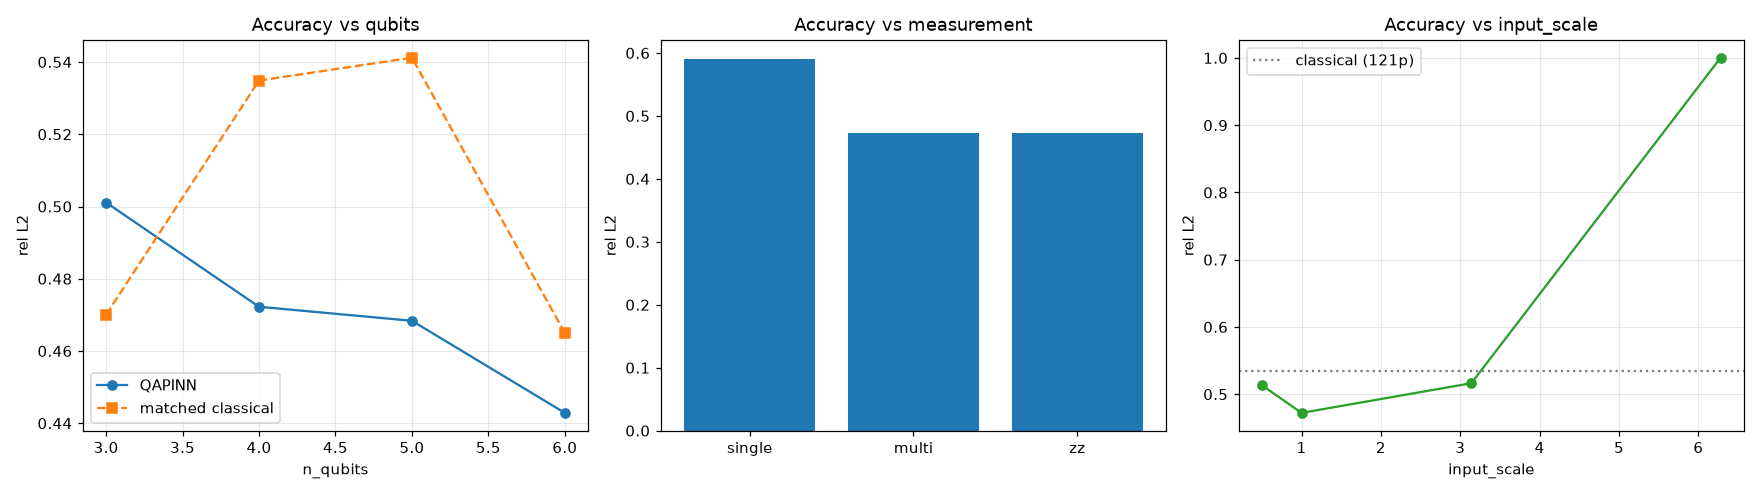
\includegraphics[width=\textwidth]{tier3_sweeps.png}
  \caption{Tier-3 sweeps: qubits (bandwidth-like), measurement (readout width vs
  type), encoding scale (optimum $+$ $2\pi$ collapse).}
  \label{fig:tier3}
\end{figure}

Five knobs split cleanly: \emph{bandwidth} knobs (depth, qubits, encoding scale)
carry the advantage up to a trainability ceiling; \emph{coefficient/readout} knobs
(entanglement, correlator measurement) do not --- the bandwidth-vs-trainability
squeeze, across five knobs.

\subsection{How the quantum layer changes the classical network}
A na\"ive comparison against a plain PINN suggested the quantum layer makes the
downstream neurons more diverse and drives larger gradients, but that comparison is
confounded (different post-net shape). We instead use a \emph{structurally
identical} classical-front-end control (CFE): the same post-net fed by
$\mathrm{Linear}(2\!\to\!w)+\tanh$ instead of the VQC. Against this fair control
(Table~\ref{tab:classical}), the effects do \emph{not} hold: accuracy is
bandwidth-gated (QAPINN ties at low depth/qubits, wins at depth 5 / 6 qubits /
heat); neuron diversity is inconsistent (classical front-end more diverse on the
depth axis, quantum more on qubits); and gradient amplification reverses at 5--6
qubits, where the QAPINN gradient variance shrinks with qubit count (a
barren-plateau signature). What survives: a bandwidth-gated advantage and a
barren-plateau signature --- the classical-side ``mechanism'' is not a clean effect.

\begin{table}[t]
  \centering \small
  \begin{tabular}{lccc}
    \toprule
    Comparison & rel-$L_2$ (Q\,/\,C) & diversity (Q\,/\,C) & grad-var $\times10^{-3}$ (Q\,/\,C) \\ \midrule
    Burgers depth-3 & 0.472 / 0.474 & 0.269 / \textbf{0.286} & \textbf{4.1} / 0.62 \\
    Burgers depth-5 & \textbf{0.424} / 0.474 & 0.236 / \textbf{0.286} & \textbf{7.1} / 0.62 \\
    Heat            & \textbf{0.006} / 0.013 & \textbf{0.272} / 0.239 & \textbf{3.2} / 0.47 \\
    Burgers 3 qubits & 0.501 / 0.496 & \textbf{0.266} / 0.241 & \textbf{1.2} / 0.26 \\
    Burgers 5 qubits & 0.468 / 0.464 & \textbf{0.312} / 0.265 & 1.1 / \textbf{5.2} \\
    Burgers 6 qubits & \textbf{0.443} / 0.467 & \textbf{0.341} / 0.269 & 0.72 / \textbf{1.9} \\ \bottomrule
  \end{tabular}
  \caption{Post-net neurons, quantum (Q) vs classical (C) front-end on the identical
  post-net. Bold $=$ larger of each pair. Single seed.}
  \label{tab:classical}
\end{table}

\begin{figure}[t]
  \centering 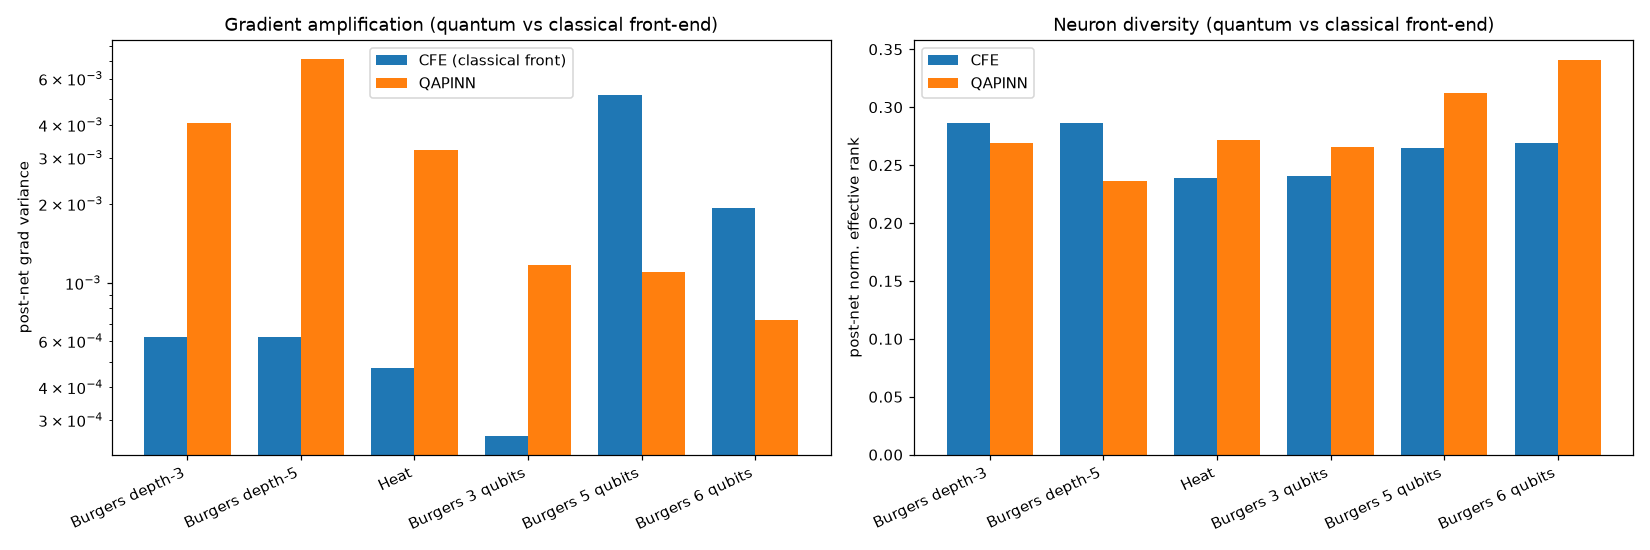
\includegraphics[width=\textwidth]{cfe_comparison.png}
  \caption{Quantum vs classical front-end on the identical post-net: gradient
  variance (left) and neuron diversity (right). Neither effect is robust across
  knobs.}
  \label{fig:classical}
\end{figure}

\subsection{Discussion}
The evidence is coherent: the quantum layer's behaviour is a \emph{bandwidth}
phenomenon (tracks depth/qubits/scale, not entanglement at fixed band, needs but is
not subsumed by a classical readout, holds up to a trainability ceiling). Against a
fair control the advantage is \emph{bandwidth-gated} and the apparent classical-side
mechanism does \emph{not} survive --- what remains is a bandwidth-gated advantage
and a barren-plateau signature in qubit count.

% ===========================================================================
\section{Current Limitations}
Hypotheses, not claims: (1) single seed --- pairwise gaps ($\sim$7\%) are within
plausible init noise; (2) undertrained, one PDE (Burgers $0.42$--$0.57$); (3) a
structural confound in the diversity comparison (16 vs 30 neurons), mitigated by
the fixed-post-net depth sweep; (4) simulation only (no shot noise / hardware).
Code verified; conclusions not yet.

% ===========================================================================
\section{Future Work and Experimental Roadmap}
\label{sec:roadmap}
The single most important next step follows from the ``undertrained'' limitation:
\emph{establish convergence before spending compute on statistics.} The revised
priority order is therefore convergence, then seeds, then breadth.

\subsection{Tier 2a --- Convergence / iteration analysis (highest priority)}
Because all current results are undertrained, every ordering may be a transient.
Iterations is nearly free as an ablation: checkpoints and the loss history from a
single long run yield every iteration point. Plan: long-train the headline
configs (baseline QAPINN, entanglement-none QAPINN, matched classical) to
$\sim$8000 iters with dense checkpoints, and re-evaluate all metrics
(accuracy, realised spectrum, entanglement, classical-side diversity/gradients)
along the trajectory. Questions: do the depth and entanglement orderings persist
at convergence? Does the slower-training QAPINN (its $k{=}1$ error halves at
iter 550 vs 75 for classical) catch up, plateau higher, or overtake? Do the
classical-side effects grow or fade? Cost: $\sim$5\,h.

\subsection{Tier 2b --- Multi-seed robustness (error bars)}
Re-run the surviving headline configs across 3--5 seeds to obtain mean $\pm$ std,
and accept a difference only if it exceeds the seed spread. Priority: the
entanglement-does-not-help result (publishable if it survives) and the
classical-side diversity/gradient effects. Cost: $\sim$10\,h.

\subsection{Tier 2c --- The classical-front-end control}
To remove the last confound from the ``diversity'' finding, add a control with an
\emph{identical} post-net but a classical $2\!\to\!4$ front-end, and compare its
post-net directly to the QAPINN's. This isolates ``quantum vs classical front-end
effect on the same classical net.'' Cost: negligible (classical).

\subsection{Tier 3 --- Remaining ablation axes and the bandwidth continuum}
\begin{itemize}[nosep]
  \item \textbf{$\nu$-sweep (bandwidth continuum):} tune Burgers viscosity from
  smooth to sharp and plot advantage vs solution bandwidth --- the continuum that
  turns two discrete regularity points (heat, Burgers) into a scaling relation.
  This directly tests whether bandwidth is a \emph{sufficient statistic} for
  advantage.
  \item \textbf{Qubits} (3--6): more bandwidth + Hilbert space (changes params;
  needs re-matching + barren-plateau watch).
  \item \textbf{Measurement:} single / multi / ZZ, and the not-yet-implemented
  \emph{probability vector} readout that the challenge explicitly requests.
  \item \textbf{input\_scale} and \textbf{loss weighting:} secondary bandwidth /
  optimisation levers (the latter drove the earlier full-quantum collapse).
  \item \textbf{Encoding scheme:} the coordinate$\to$qubit map (round-robin vs
  split vs all-on-all).
\end{itemize}

\subsection{Tier 4 --- Real CFD and mathematical depth}
\begin{itemize}[nosep]
  \item \textbf{Lid-driven cavity (2-D incompressible Navier--Stokes):} the
  real-world CFD case the judges reward; the PDE-agnostic bench already supports
  multi-output, multi-equation systems. Literature suggests quantum may
  \emph{lose} here --- a valid ``what is lost'' finding.
  \item \textbf{Fourier coefficient reachability (Mhiri):} measure realised
  \emph{coefficients} vs the reference, not just the frequency support, to test
  whether the depth-5 bandwidth shortfall (max freq 4, not 5) is the coefficient
  constraint biting.
  \item \textbf{Barren-plateau / trainability study:} systematic gradient-variance
  vs qubits/depth over many random initialisations; relation to the
  ``black-hole'' collapse.
\end{itemize}

\subsection{The deliverable --- design methodology}
The end goal (challenge Task 4) is a validated chain: \emph{cheap proxy}
(Reynolds/$\nu$, or a coarse classical/FEA solve) $\to$ estimated solution
bandwidth $\to$ prescribed circuit (qubits, depth, encoding). Validation uses exact
solutions; deployment uses the proxy, resolving the circularity of ``needing the
solution to size the circuit.''

\begin{table}[t]
  \centering \small
  \begin{tabular}{llll}
    \toprule
    Tier & Content & Est.\ compute & Promotes \\ \midrule
    2a & convergence (iterations) & $\sim$5\,h & undertraining $\to$ converged \\
    2b & 3--5 seeds on headlines & $\sim$10\,h & hypotheses $\to$ error-barred \\
    2c & classical-front-end control & $\sim$0 & removes diversity confound \\
    3 & $\nu$-sweep + remaining knobs & $\sim$15\,h & mechanism $\to$ sufficiency \\
    4 & real CFD + coefficient/BP analysis & TBD & breadth + math rigour \\
    \bottomrule
  \end{tabular}
  \caption{Experimental roadmap with rough compute cost (single laptop,
  \texttt{default.qubit}). \texttt{lightning.qubit} may accelerate the simulation
  but currently breaks the higher-order autograd needed for $u_{xx}$.}
  \label{tab:roadmap}
\end{table}

% ===========================================================================
\section{What Is Currently Left Out (Scope Boundaries)}
\label{sec:leftout}
For transparency, the present study explicitly does \emph{not} yet include:
\begin{itemize}[nosep]
  \item \textbf{Statistics:} no repeated seeds, no error bars, no significance
  tests --- every result is a single point estimate.
  \item \textbf{Convergence:} nothing trained to convergence; all Burgers results
  are Adam-only and undertrained.
  \item \textbf{Breadth of PDEs:} only Burgers and heat; no real CFD (cavity),
  no $\nu$-continuum.
  \item \textbf{Full VQC knob set:} qubits, measurement (incl.\ probability
  vector), input\_scale, encoding scheme, and loss weighting are not yet ablated;
  Tier 1 covered only depth, entanglement, and post-net width.
  \item \textbf{Coefficient-level Fourier analysis:} we measure realised frequency
  \emph{support}, not the realised \emph{coefficients} vs their reachable set
  (Mhiri).
  \item \textbf{Trainability theory:} the black-hole collapse and barren plateaus
  are discussed but not systematically measured on QAPINNs.
  \item \textbf{Hardware / noise:} statevector simulation only; no shot noise, no
  device runs; ``parameter reduction'' is not ``resource reduction''
  ($\sim$85$\times$ slower in simulation).
  \item \textbf{Design methodology:} the proxy$\to$bandwidth$\to$circuit rule is
  designed but not yet validated end-to-end.
\end{itemize}

% ===========================================================================
\section{Conclusion}
We have a verified bench, a five-dimension XAI suite, and a coherent set of
single-seed hypotheses: the quantum layer's behaviour is a bandwidth phenomenon
(not entanglement). Against a structurally-identical classical-front-end control the
advantage is bandwidth-gated, and the apparent classical-side mechanism does not
survive --- what remains is a bandwidth-gated accuracy advantage and a
barren-plateau signature in qubit count. The immediate next step is the convergence
(Tier 2a) analysis, followed by multi-seed error bars (Tier 2b), after which the
surviving hypotheses become claims and the design methodology can be validated.

% ===========================================================================
\begin{thebibliography}{9}
\small
\bibitem{raissi} M.~Raissi, P.~Perdikaris, G.~E.~Karniadakis. \emph{Physics-informed deep learning (Part I)}, 2019.
\bibitem{schuld} M.~Schuld, R.~Sweke, J.~J.~Meyer. \emph{Effect of data encoding on the expressive power of variational QML models}. Phys.\ Rev.\ A \textbf{103}, 032430 (2021).
\bibitem{dqc} O.~Kyriienko, A.~E.~Paine, V.~E.~Elfving. \emph{Solving nonlinear DEs with differentiable quantum circuits}. Phys.\ Rev.\ A \textbf{103}, 052416 (2021).
\bibitem{qapinn} J.~Shah, R.~Lineswala, A.~Chopra. \emph{Benchmarking QA-PINN for CFD}. IEEE QCE 2024.
\bibitem{mhiri} S.~Mhiri et al. \emph{Constrained and Vanishing Expressivity of Quantum Fourier Models}. Quantum \textbf{9}, 1847 (2025).
\bibitem{qcpinn} A.~Farea, M.~Khan. \emph{QCPINN: Quantum-Classical PINNs for PDEs}. MLST (2025).
\bibitem{maxwell} Chen et al. \emph{Quantum PINNs for Maxwell's Equations}. Quantum Machine Intelligence (2026).
\end{thebibliography}

\end{document}
